% Sablon pentru realizarea lucrarii de licenta, conform cu recomandarile
% din ghidul de redactare:
% - https://fmi.unibuc.ro/finalizare-studii/
% - https://drive.google.com/file/d/1xj9kZZgTkcKMJkMLRuoYRgLQ1O8CX0mv/view

% Multumiri lui Gabriel Majeri, acest sablon a fost creat pe baza
% codului sursa a lucrarii sale de licenta. 
% Codul sursa: https://github.com/GabrielMajeri/bachelors-thesis
% Website: https://www.gabrielmajeri.ro/
%
% Aceast sablon este licentiat sub Creative Commons Attribution 4.0 International License.

\documentclass[12pt, a4paper]{report}

% Suport pentru diacritice și alte simboluri
\usepackage{fontspec}

% Suport pentru mai multe limbi
\usepackage{polyglossia}

% Setează limba textului la română
\setdefaultlanguage{romanian}
% Am nevoie de engleză pentru rezumat
\setotherlanguages{english}

% Indentează și primul paragraf al fiecărei noi secțiuni
\SetLanguageKeys{romanian}{indentfirst=true}

% Suport pentru diferite stiluri de ghilimele
\usepackage{csquotes}

\DeclareQuoteStyle{romanian}
  {\quotedblbase}
  {\textquotedblright}
  {\guillemotleft}
  {\guillemotright}

% Utilizează biblatex pentru referințe bibliografice
\usepackage[
    maxbibnames=50,
    sorting=nty
]{biblatex}

\addbibresource{bibliography.bib}

% Setează spațiere inter-linie la 1.5
\usepackage{setspace}
\onehalfspacing

% Modificarea geometriei paginii
\usepackage{geometry}

% Include funcțiile de grafică
\usepackage{graphicx}
% Încarcă imaginile din directorul `images`
\graphicspath{{./images/}}

% Listări de cod
\usepackage{listings}

% Linkuri interactive în PDF
\usepackage[
    colorlinks,
    linkcolor={black},
    menucolor={black},
    citecolor={black},
    urlcolor={blue}
]{hyperref}

% Simboluri matematice codificate Unicode
\usepackage[warnings-off={mathtools-colon,mathtools-overbracket}]{unicode-math}

% Comenzi matematice
\usepackage{amsmath}
\usepackage{mathtools}

% Formule matematice
\newcommand{\bigO}[1]{\symcal{O}\left(#1\right)}
\DeclarePairedDelimiter\abs{\lvert}{\rvert}

% Suport pentru rezumat în două limbi
% Bazat pe https://tex.stackexchange.com/a/70818
\newenvironment{abstractpage}
  {\cleardoublepage\vspace*{\fill}\thispagestyle{empty}}
  {\vfill\cleardoublepage}
\renewenvironment{abstract}[1]
  {\bigskip\selectlanguage{#1}%
   \begin{center}\bfseries\abstractname\end{center}}
  {\par\bigskip}

% Suport pentru anexe
\usepackage{appendix}

% Stiluri diferite de headere și footere
\usepackage{fancyhdr}

% Metadate
\title{Titlul lucrării de licență}
\author{Florete Fabian-Andrei}

% Generează variabilele cu @
\makeatletter

\begin{document}

% Front matter
\cleardoublepage
\let\ps@plain

% Pagina de titlu
\begin{titlepage}

% Redu marginile
\newgeometry{left=2cm,right=2cm,bottom=1cm}

\begin{figure}[!htb]
    \centering
    \begin{minipage}{0.2\textwidth}
        
\includegraphics[width=\linewidth]{logo-ub.png}
    \end{minipage}
    \begin{minipage}{0.5\textwidth}
        \large
        \vspace{0.2cm}
        \begin{center}
            \textbf{UNIVERSITATEA DIN BUCUREȘTI}
        \end{center}
        \vspace{0.3cm}
        \begin{center}
            \textbf{
                FACULTATEA DE \\
                MATEMATICĂ ȘI INFORMATICĂ
            }
        \end{center}
    \end{minipage}
    \begin{minipage}{0.2\textwidth}
        
\includegraphics[width=\linewidth]{logo-fmi.png}
    \end{minipage}
\end{figure}

\begin{center}
\textbf{SPECIALIZAREA INFORMATICĂ}
\end{center}

\vspace{1cm}

\begin{center}
\Large \textbf{Lucrare de licență}
\end{center}

\begin{center}
\huge \textbf{\MakeUppercase{\@title}}
\end{center}

\vspace{3cm}

\begin{center}
\large \textbf{Absolvent \\ \@author}
\end{center}

\vspace{0.25cm}

\begin{center}
\large \textbf{Coordonator științific \\ Conf. Dr. Sergiu Nisioi}
\end{center}

\vspace{2cm}

\begin{center}
\Large \textbf{București, Iunie 2025}
\end{center}
\end{titlepage}
\restoregeometry
\newgeometry{
    margin=2.5cm
}

\fancypagestyle{main}{
  \fancyhf{}
  \renewcommand\headrulewidth{0pt}
  \fancyhead[C]{}
  \fancyfoot[C]{\thepage}
}

\addtocounter{page}{1}

% Rezumatul
\begin{abstractpage}

\begin{abstract}{romanian}
Creierul uman constituie una dintre cele mai complexe și mai promițătoare arii de cercetare. Și, contrar faptului că a fost studiat intens de-a lungul timpului, încă nu avem un model destul de clar al modului în care acesta funcționează.

În această lucrare de licență am urmărit să explorez, să evaluez și să compar cât mai mulți algoritmi legați de interpretarea semnalelor emise de creier. Scopul principal este de a vedea gradul de interpretabilitate generat de diverși stimuli de scurtă durată. Lucrarea mea se diferențiază de restul lucrărilor din domeniul ERP prin tipul datelor folosite și prin specificitatea subiecților. Astfel, datele mele provin de la oameni specializați, și anume arhitecți ce au privit imagini specifice domeniului, mai exact coloane generate artificial.

Pe parcursul lucrării am implementat și comparat sistematic algoritmi documentați în literatura de specialitate.
\end{abstract}

\begin{abstract}{english}
The human brain represents one of the most complex and promising areas of research. And, although it has been intensely  studied throughout the years, we still do not have an accurate model of the way it functions.

In this thesis, I aimed to explore, evaluate and compare a wide range of algorithms related to the interpretation of brain-emitted signals. The main objective is to asses the degree of interpretability elicited by various short-duration stimuli. My work differs from the existing literature in the ERP domain via the type of data used and the specificity of the subjects. The data used comes from specialized subjects, more particularly architects that have been shown images specific to their domain, specifically, artificially generated columns.

Throughout the study, I systematically implemented and compared algorithms documented in the scientific literature.
\end{abstract}

\end{abstractpage}

\tableofcontents

% Main matter
\cleardoublepage
\pagestyle{main}
\let\ps@plain\ps@main

\chapter{Introducere}

\section{Context și motivație}
EEG-ul, sau Electroencefalograma, reprezintă o modalitate sigură și non-invazivă de a măsura activatea electromagnetică a creierului. Această măsurare se face printr-o cască ce conține mai mulți electrozi. Fiecare electrod în parte măsoara activiatea creierului in Volți. Ele au aplicații intr-o multitudine de domenii. Cele mai folosite cazuri în literatura de specialitate sunt: detectarea fazelor somnului, a simptomelor epilepsiei, a sindromului Alzheimer, a diferitelor emoții puternice, precum tristețe, frică, fericire și, în domeniul de Brain-Computer interface, care se concentrează pe decodarea semnalelor creierului asociate cu mișcarea membrelor.
De-a lungul anilor, cercetătorii au obținut rezultate din ce in ce mai bune în domeniul clasificarii emoțiilor induse de un stimul vizual. Daca în anul 2016 modelele state of the art ce se bazau pe SVM-uri ajungeau la o acuratețe de 73\%\cite{ATKINSON201635}, în anul 2020, modele precum TSception, ce se bazează pe Rețele neuronale ating acuratețe de peste 86\%\cite{TSception}. 

Totuși, în majoritatea cazurilor, stimulii induși sunt cauzați fie de evenimente de lungă durată: video-uri, ore intregi de somn, fie de evenimente binare, având clase target sau non-target.

\section{Obiectivele Lucrării}
Scopul lucrării este de a vedea dacă putem clasifica stimuli vizuali, prezentați pe parcursul unei durate scurte, în funcție de reacția unui participant, dispunând de 3 categorii de răspuns: pozitiv, neutru, negativ.


\def\totalEpoci{0}
\def\totalEpociTestare{0}
\def\totalEpociValentaPozitiva{0}
\def\totalEpociValentaNegativa{0}
\def\totalEpociValentaNeutra{0}
\def\crestereAcurateteAutoReject{0}
\def\nrParticipantiAntrenare{0}
\def\nrParticipantiValidare{0}
\def\nrParticipantiTestare{0}

\usepackage{float}

\chapter{Metodologia}

\section{Setul de date}
\subsection{Preluarea datelor și formatul lor}
Datele constau în 26 de fișiere excel reprezentând subiecții experimentului. Fiecare fișier conține înregistrările corespunzătoare a 21 de electrozi plasați de-a lungul capului. Ei au măsurat activitatea creierului cu o frecvență de 300 Hz. Există și un canal de referință Pz care a fost folosit pentru a calibra măsurătorile. Astfel, el nu apare în setul de date. Corespunzător fiecarui fișier, mai există un fișier de quizz care reprezintă notele acordate de subiect fiecărei imagini văzute. Imaginile sunt notate pe 3 criterii V(Valence/Valență), A(Arousal/Excitare) și D(Dominance/Dominanță). Notele stimulilor sunt discretizate in 3 categorii: stimul negativ (note de la 1 la 3), stimul neutru (note de la 4 la 6) și stimul pozitiv (note de la 7-10). Scopul este astfel prezicerea categoriei de stimul provocat de o imagine.
\setlength{\abovecaptionskip}{0pt}
\setlength{\belowcaptionskip}{0pt}
\clearpage
\begin{figure}[h]
    \centering
    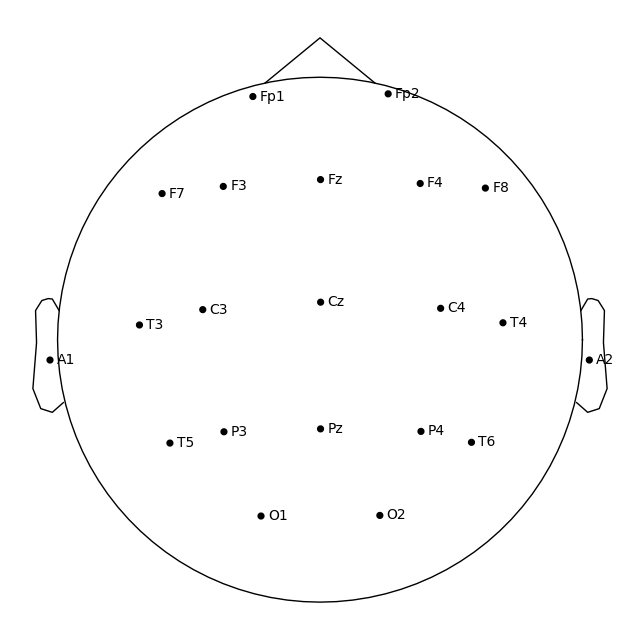
\includegraphics[width=8cm]{images/Sensor_positions_(eeg).png}
    \caption{Pozițiile electrozilor la nivelul capului}
    \label{fig:sensor_positions}
\end{figure}
Datele din formatul brut sunt încărcate folosind libraria Pandas \cite{reback2020pandas} din Python. Pe urmă, am mai adăugat coloane specifice lable-urilor experimentului. Mai departe, am transformat datele în format .FIF și le-am încărcat în format de EEG-uri Raw utilizând MNE \cite{MNE}.

\section{Preprocesarea datelor}
Înainte de introduce datele în modele, acestea trebuie curățate. În primul rând, nu toate frecvențele sunt relevante pentru task-urile de clasificare. Multe pot proveni din zgomot de fond sau interferențe electrice, precum zgomotul generat de rețeaua electrică sau imperfecțiunea electrozilor. 

% Toata partea de preprocesare este parametrizată pentru a permite cautarea valorilor optime.

% \setlength{\abovecaptionskip}{0pt}
% \setlength{\belowcaptionskip}{0pt}
% \begin{figure}
%     \centering
%     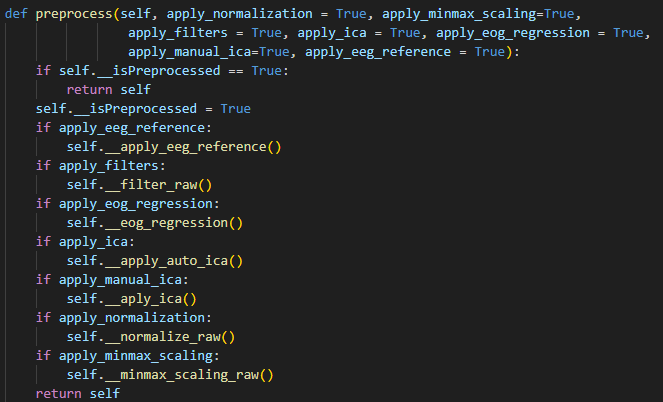
\includegraphics[width=10cm]{images/parametrizare.png}
%     \caption{Enter Caption}
%     \label{fig:enter-label}
% \end{figure}


\subsection{Filtrare, interpolare, ICA}

Literatura de specialitate sugerează să filtram datele astfel încât să păstram doar frecvențele între 4-45 Hz. Am folosit astfel un filtru bandpass. Modul de functionare al acestuia este următorul: este creeat un filtru în domeniul frecvențelor. Acest filtru este transpus în domeniul timp. Din semnalul original sunt luate bucăți segmentate. Ele sunt înmulțite cu o fereastră hamming pentru a elimina fenomenul de spectral leakage. Bucata segmentată este trecută prin operația de convoluție cu filtrul original și astfel este obținut un semnal filtrat.

\setlength{\abovecaptionskip}{0pt}
\setlength{\belowcaptionskip}{0pt}
\clearpage
\begin{figure}[h]
    \centering
    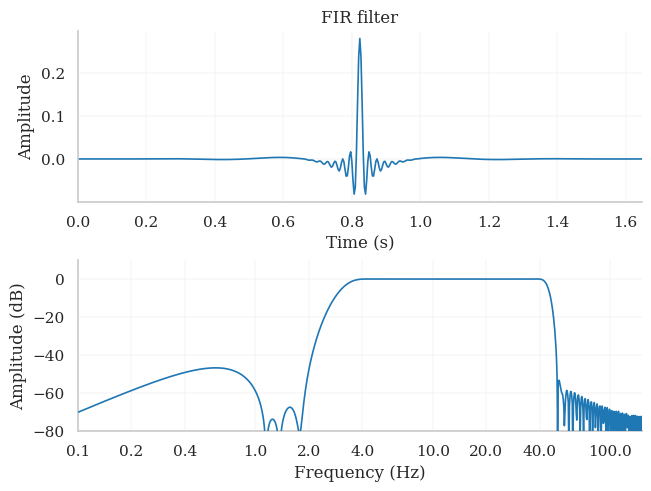
\includegraphics[width=12cm]{filtru.png}
    \caption{Filtrul bandpass folosit}
    \label{fig:vizualizare_filtru}
\end{figure}

Urmatoarea preprocesare aplicată este interpolarea canalelor corupte. Semnalul canalelor marcate ca fiind corupte este înlocuit prin interpolarea canalelor vecine acestuia. Mai departe, am aplicat tehnica de ICA(Independent Component Analysis) pentru a elimina clipirile din canalele Fp1 și Fp2 ce aveau reverberații și asupra celorlalte canale. Tehnica se bazeaza pe descompunerea semnalelor într-un număr de componente specificate. Pe urmă, componentele ce se află în zona ochilor sau trec de un anumit threshold sunt eliminate, fie manual, prin selecția componentelor ce indica activitate în zona ochilor, fie automat printr-un threshold selectat.

\vspace{1em}
\begin{figure}[h]
    \centering
    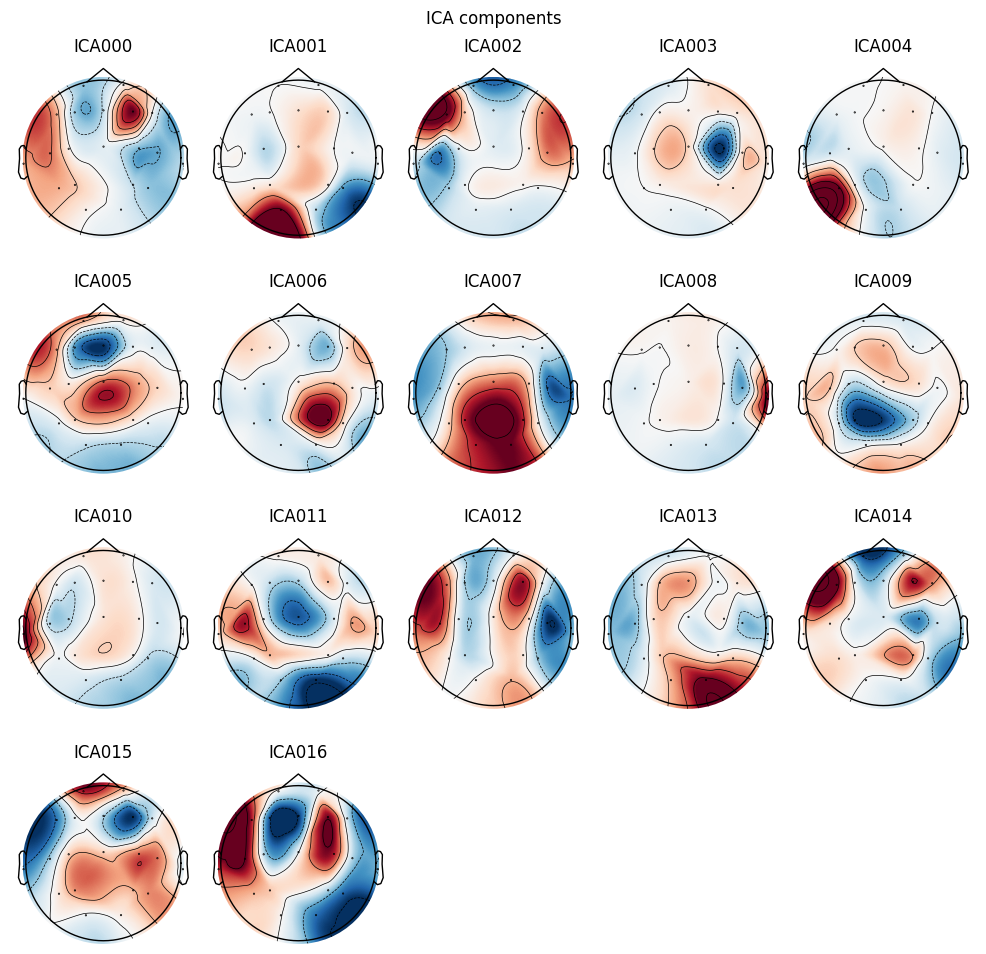
\includegraphics[width=8cm]{images/ica_components.png}
    \caption{Descompunerea ICA}
    \label{fig:vizualizare_filtru}
\end{figure}


\setlength{\abovecaptionskip}{0pt}
\setlength{\belowcaptionskip}{0pt}
\clearpage

\begin{figure}[!htb]
    \centering
    \begin{minipage}{\textwidth}
        \centering
        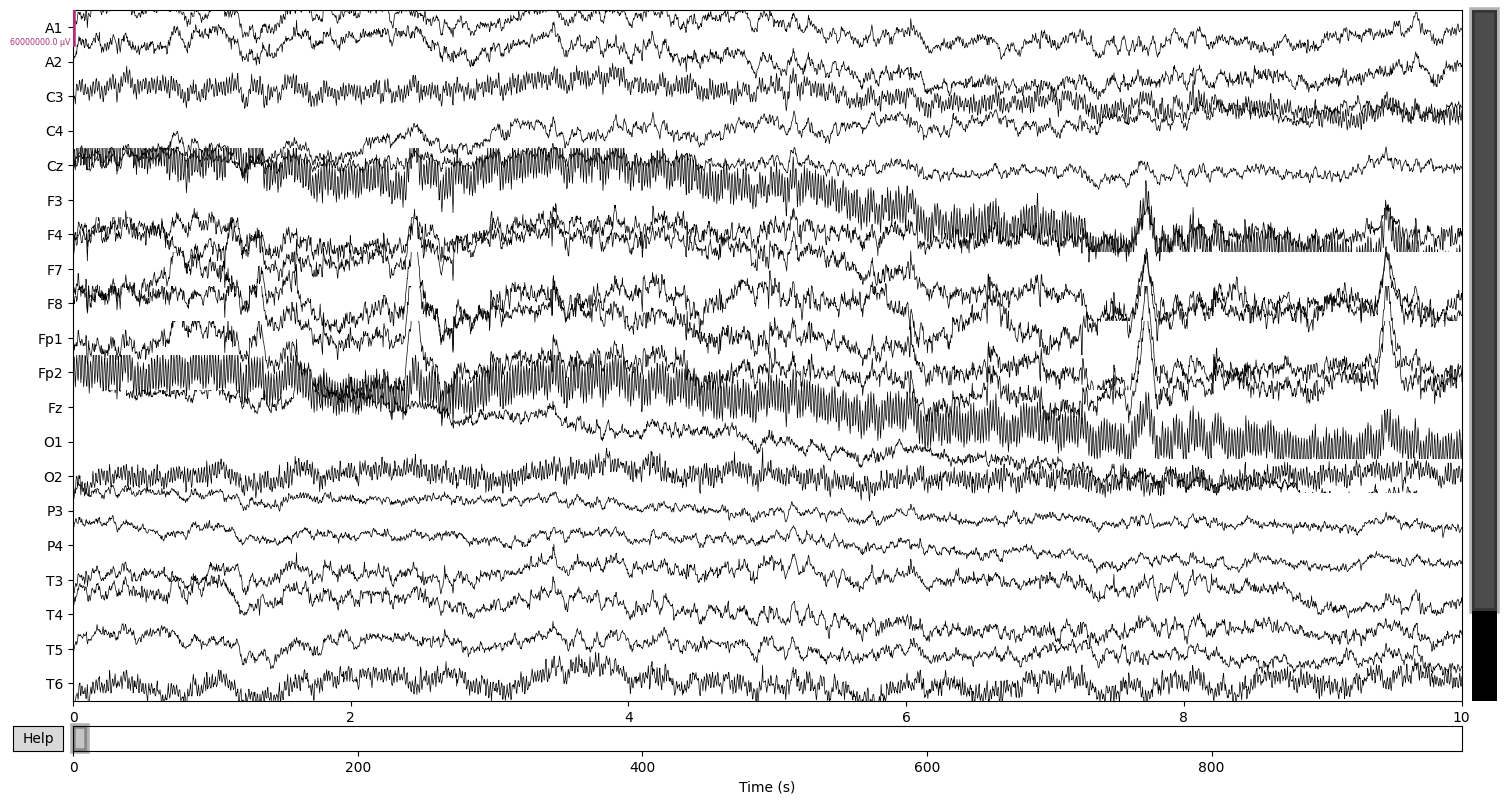
\includegraphics[width=0.8\textwidth]{images/raw_inainte.png}
        \label{fig:raw_inainte}
    \end{minipage}
    \vspace{0.5cm}
    \begin{minipage}{\textwidth}
        \centering
        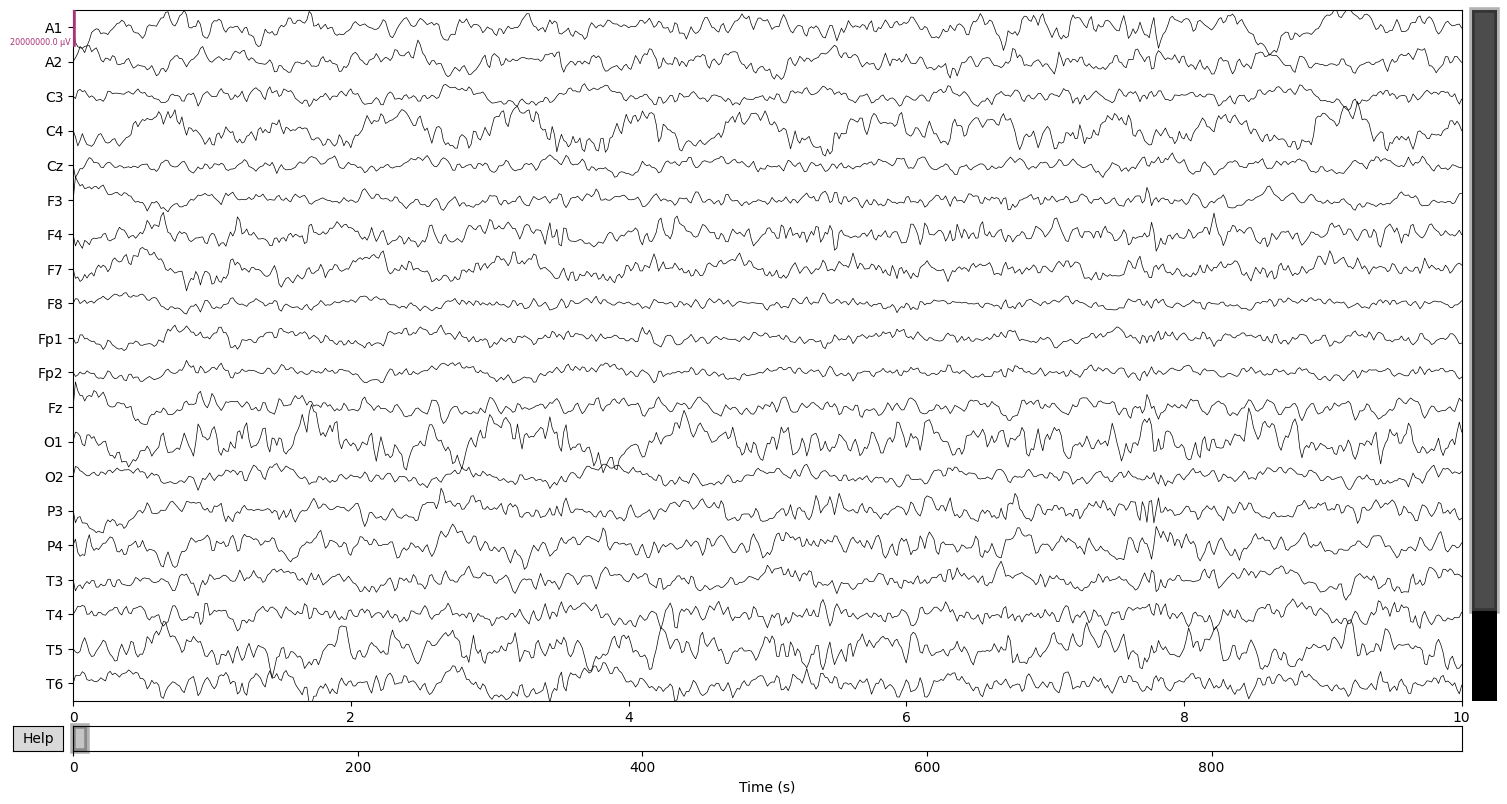
\includegraphics[width=0.8\textwidth]{images/raw_dupa.png}
        \label{fig:raw_dupa}
    \end{minipage}
    \caption{Semnalul înainte și după filtrare}
    \label{fig:raw_inainte_dupa}
\end{figure}

Calitatea datelor a fost semnificativ îmbunătățită. Am eliminat zgomotul cauzat de clipiri, drift-urile și frecvențele înalte.

\subsection{Separare în epoci, AutoReject}

Mai departe, pentru a avea date pentru clasificare, am împărțit semnalul continuu în epoci. O epocă reprezintă o fereastră mai mică din semnalul original. Aceasta este extrasa din semnalul continuu cu ajutorul unui canal auxiliar ce conține indexul stimulului prezentat sau 0 daca în acel moment nu este prezentat niciun stimul. Pentru a elimina eventualele probleme cauzate de mărimi diferite ale datelor, pentru fiecare epocă am luat și 0.2 secunde de semnal de dinaintea evenimentului de trigger(afișarea imaginii). Pe acesta le-am folosit pe post de baseline pentru a scădea din restul semnalului valoarea lor. Centrând astfel începutul și sfârșitul epocii în jurul lui 0.

\setlength{\abovecaptionskip}{0pt}
\setlength{\belowcaptionskip}{0pt}
\clearpage
\begin{figure}
    \centering
    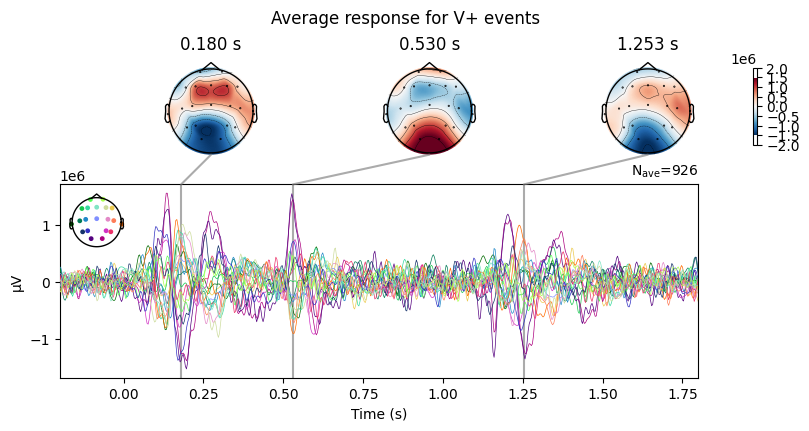
\includegraphics[width=17cm]{epoca_valenta_pozitiva.png}
    \caption{Raspunsul mediu al tuturor subiecților pentru o imagine cu valență pozitivă}
    \label{fig:enter-label}
\end{figure}

Totuși, nu toate epocile sunt bune. Unele dintre ele încă au imperfecțiuni și pot contamina datele de antrenare, așa că ele trebuie aruncate. Pentru a automatiza procesul de găsire și eliminare a epocilor corupte am folosit AutoReject\cite{AutoReject}. Această librarie găsește atât epoci corupte cât și canale corupte în epocile valide. Impactul aplicării acestui proces a fost creșterea acurateții cu $\crestereAcurateteAutoReject$\% pentru cel mai bun model folosit.

\vspace{1em}
\begin{figure}[h]
    \centering
    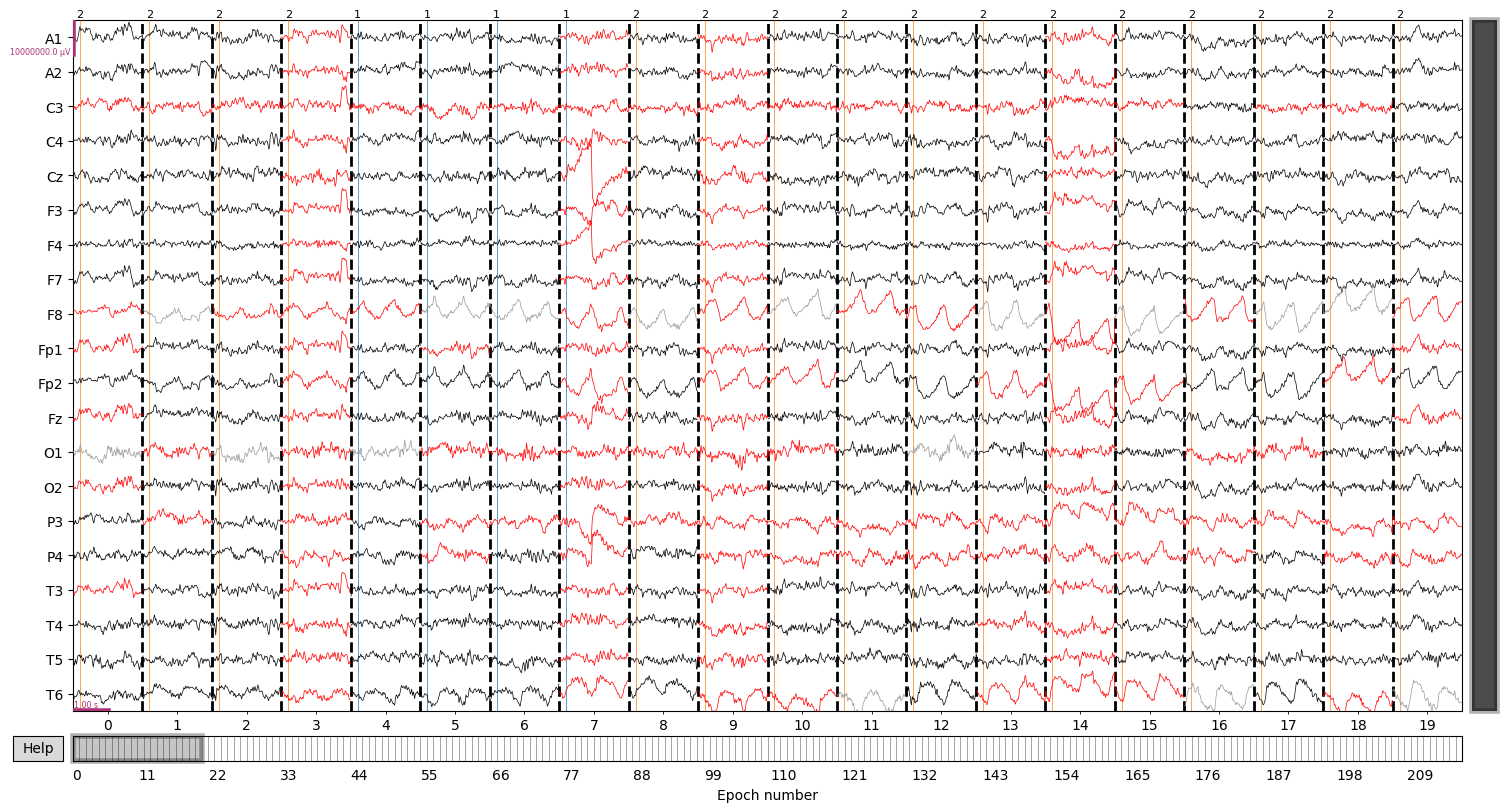
\includegraphics[width=0.8\textwidth]{images/rezultat_autoreject.png}
    \caption{Epocile eliminate de AutoReject}
    \label{fig:vizualizare_filtru}
\end{figure}

\subsection{Balansarea claselor și modul de testare}

În total am dispus de $\totalEpoci$ epoci provenite din cei 26 de subiecți. Din rândul tuturor epocilor, $\totalEpociValentaNegativa$ au valență negativă, $\totalEpociValentaNeutra$ neutră și $\totalEpociValentaPozitiva$ pozitivă. Numărul poate varia, deoarece AutoReject conține și componente non-deterministe. Pentru a testa performanța modelelor, am utilizat cross-validation asupra celor 26 participanți în felul următor: $\nrParticipantiAntrenare$ de participanți au fost extrași pentru antrenare, $\nrParticipantiValidare$ pentru validare și încă $\nrParticipantiTestare$ pentru testare.

Putem observa rapid faptul că epocile nu sunt distribuite după etichetă în mod egal. Dacă modelul ar prezice numai valență neutră, ar avea acuratețe mai mare decât dacă ar prezice la întâmplare. Pentru a aborda problema imbalansului claselor am folosit 2 abordări. Prima este de a calcula weight-urile claselor, transmițându-le mai departe la clasificator. A doua este de a utiliza metoda SMOTE\cite{imblearn} pentru a genera date sintetice.

\section{Extragerea caractersiticilor}
În domeniul clasificării semnalelor EEG există 2 paradigme pentru extragerea caracteristicilor. Prima este de a trata semnalul EEG ca fiind o serie de timp. Datele de eșantioanare ale semnalului fiind trimise mai departe spre model ca input. A doua este de a trata semnalului drept o sursă statistică de feature-uri, de unde sunt extrase caracteristici sintetice. Acestea sunt sub forma de medii, proprietăți spectrale, sau date din geometria Riemann, care mai apoi sunt transmise unui model.

\subsection{Datele drept semnale EEG}
După cum am spus, semnalul EEG are 20 de canale. Totuși, dintre acestea, nu toate sunt relevante. Pentru a găsi cele mai relevante canale, în primul rand am transpus semnalul in domeniul timp-frecvență utilizând morlet wavelets. Am aplicat asta pentru toate epocile și astfel am obținut inter-trial coherence-ul(ITC). ITC ul îmi arată asemănarea în descompunerea din domeniul timp-frecvență a epocilor.

\setlength{\abovecaptionskip}{0pt}
\setlength{\belowcaptionskip}{0pt}
\clearpage
\begin{figure}[h]
    \centering
    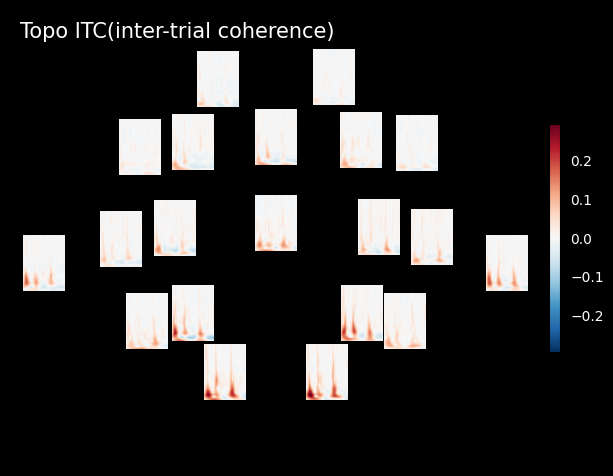
\includegraphics[width=0.6\textwidth]{images/itc_epochs.png}
    \caption{Coerența ITC}
    \label{fig:enter-label}
\end{figure}

Putem observa că diagrama are o dispunere asemănătoare cu cea a plotării electrozilor pe creier (Figura 2.1). Din această diagramă observăm importanța fiecărui canal în timpul unei epoci. Astfel, de exemplu, canalele Fp1 și Fp2 nu oferă la fel de multă informație comparativ cu O1 sau O2. Canalele alese de mine ca fiind relevante au fost: O1, O2, P3, P4, A1, A2, T5, T6. Alegând un subset de canale din cele inițiale, am mărit viteza cu care am procesat datele cu 36\%, precum și acuratețea modelului cu 3-4\%.

\vspace{1em}
\begin{figure}[!h]
    \centering
    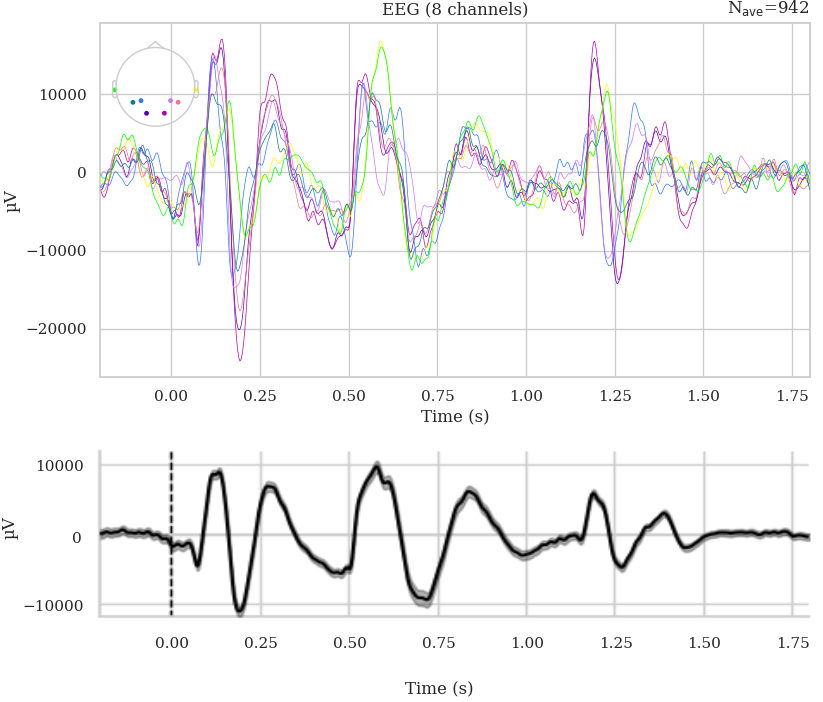
\includegraphics[width=1\linewidth, height=10cm, keepaspectratio=false]{P300_combined.png}
    \caption{ERP-ul canalelor selectate}
    \label{fig:enter-label}
\end{figure}

Un alt rezultat al alegerii unui subset de canale a fost faptul că, am reușit să apropii evenimentul de unul asemănător unuia de tip P300\cite{P300}, fiind bine cunoscut și studiat în neuroștiință. Teoria spune că, odată prezentat un stimul unui participant, răspunsul cognitiv apare la aproximativ 300 de milisecunde după evenimentul declanșator. În cazul meu, observăm că aproximativ după 0.3 s de la afișarea stimulului (momentul 0) apare un vârf, fiind precedat și antecedat de 'văi'. Prima vale are denumirea de P200, iar a doua de P300. Această dispunere a semnalului confirmă faptul că preprocesările făcute nu au alterat semnificația semnalului. %În plus, dispunerea semnalului sub forma P300 mi-a permis sa abordez și metode de transfer-learning pe seturi mai mari de date și cu mai mulți electrozi.

\vspace{1em}
\begin{figure}[h]
    \centering
    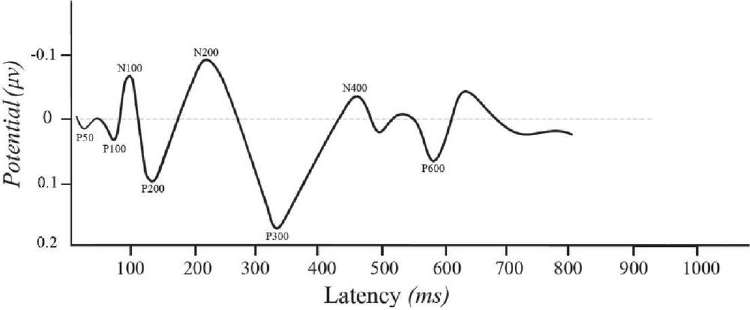
\includegraphics[width=0.9\linewidth]{P300_theory.jpg}
    \caption{Evenimentele asociate unui ERP\cite{P300_image}}
    \label{fig:enter-label}
\end{figure}


\subsection{Datele drept caracteristici statistice și descompuneri în domeniul frecvențelor}

O altă abordare a extragerii caracteristicilor o reprezintă datele statistice și spectrale din semnalul EEG. Pentru a extrage caracteristicile semnalului am utilizat mne-features\cite{mne-features}. Librăria are în total 30 de tipuri de feature-uri. Pentru a le extrage pe cele mai bune am utilizat ideea prezentă în http://refhub.elsevier.com/S0957-4174(15)00753-8/sbref0009. Și anume folosirea algoritmilor genetici împreuă cu un clasificator liniar pentru a alege o submulțime de feature-uri din cea inițiala.

------------TO BE CONTINUED AICI------------

\subsection{Datele drept feature-uri geometrice Riemann}
Alte modalități, care au recâștigat popularitate recent, constau în folosirea geometriei Riemann. Asupra datelor este aplicat algoritmul de denoising XDAWN\cite{xdawn}, urmând, pe urmă, ca semnalul să fie transpus într-un spațiu geometric Riemann. Pentru a implementa acești algoritmi m-am folosit de librăria pyRiemann\cite{pyriemann}. Algoritmii ce se folosesc de acest principiu și pe care i-am implementat și testat la rândul meu sunt: XDAWNCov + TS + SVM\cite{xdawncovtssvm} și XDAWN + LDA\cite{xdawnlda}. Benchmark-urile MOABB\cite{moabb}  arată ca aceaste două metode obțin cele mai bune performanțe pentru stimulii de tip P300. Pornind de la acești algoritmi, am adapatat unii pași, obținând, pe cazuri specifice, rezultate mai bune.

\section{Modele de clasificare}
Privind abordarea modelelor am ales să încerc cât mai multe modele, pornind de la simple clasificatoare liniare, precum SVM-uri din scikit-learn\cite{scikit-learn} și până la rețelele convoluționale din braindecode\cite{braindecode}. De asemenea, am creat, utilizând keras\cite{keras}, și modele proprii pentru un mai bun control asupra complexității și funcționalității modelului.
\subsection{Modele clasice din scikit-learn}
Pentru a evalua modelele clasice, prima dată am trecut datele de dimensiune(7, 601) adică 7 canale, fiecare canal având 601 puncte de discretizare (aceste 601 puncte provin de la frecvența înregistrărilor de 300 x 2 secunde ce reprezintă durata unei epoci) prin operația de flatten, astfel încât input-ul meu să fie 1-dimensional. Pe urmă, am normalizat datele și le-am încadrat în intervalul (0, 1) utilizând StandardScaler. În final, fiecare input reprezintă un vector cu 4207 caracteristici.

\vspace{1em}
\begin{figure}[h]
    \centering
    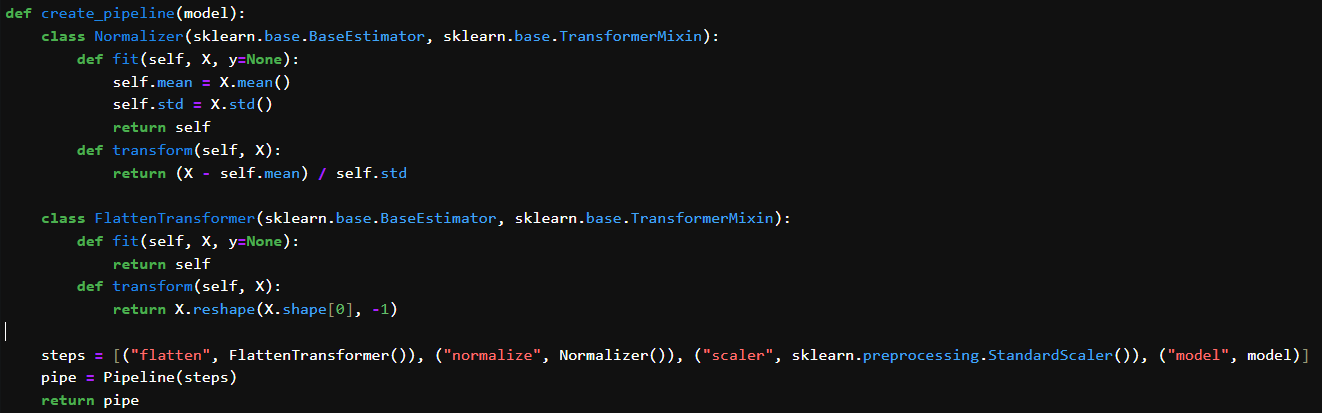
\includegraphics[width=1\linewidth]{pipeline_modele_clasice.png}
    \caption{Pipeline pentru modelele clasice}
    \label{fig:enter-label}
\end{figure}

Utilizând acest pipeline, am putut să compar sistematic mai multe tipuri de modele. Pentru a evalua performanța modelelor, am utilizat f1-score și accuracy. Pentru a lua în calcul imbalansul claselor, am creat date sintetice utilizând metoda de oversampling SMOTE. %Pentru cel mai bun model din punctul de vedere al f1-score și accuracy am făcut mai departe un classification report. %

\clearpage
\vspace{1em}
\begin{figure}[h]
    \centering
    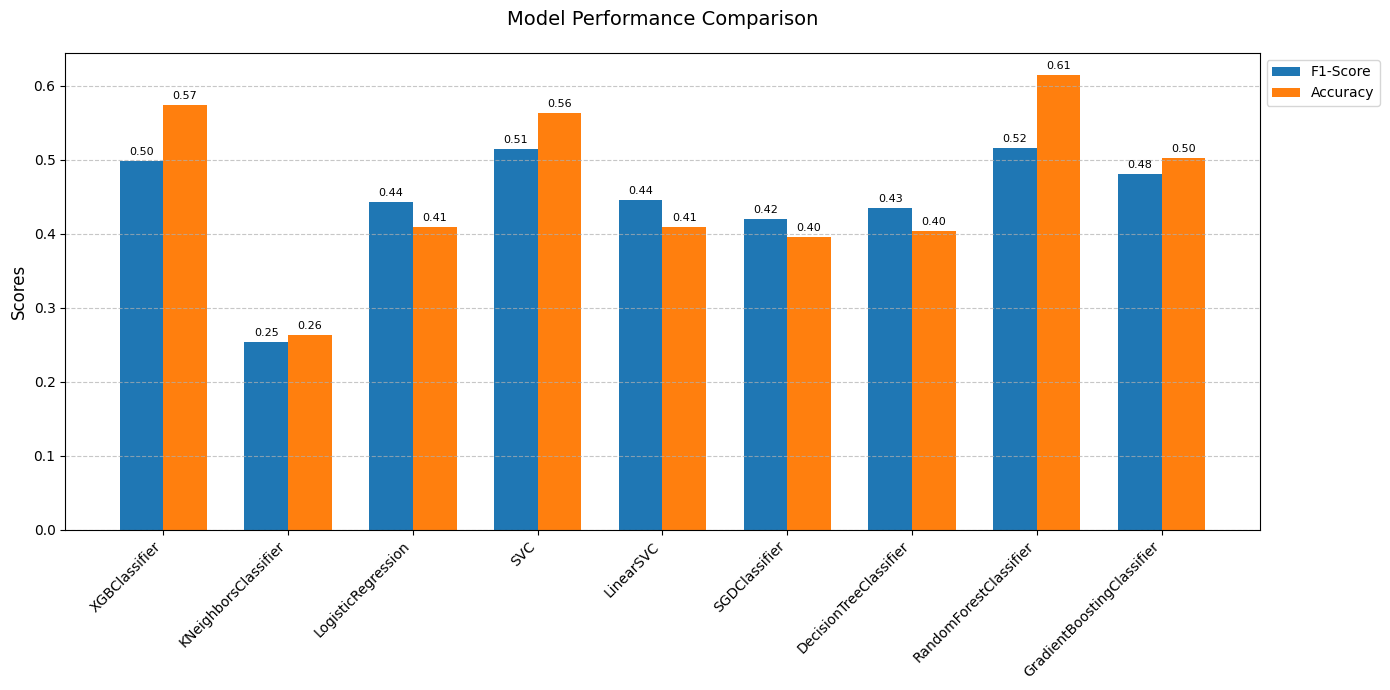
\includegraphics[width=1\textwidth]{images/comparatie_modele_clasice_unweighted.png}
    \caption{Performanța modelelor clasice}
    \label{fig:enter-label}
\end{figure}

Mai departe, pentru a încerca abordarea bazată pe caracteristici statistice și spectrale, am utilizat mne-features. Pentru a extrage un subset din feature-urile totale, am utilizat o librărie specializată în rularea algoritmilor genetici, și anume pygad \cite{pygad}. Pentru funcția de fitness, am folosit un tuplu format din f1-score și balanced-accuracy.

------------DE ADAUGAT AICI REZULTATELE RULARII ALG GENETIC------------

\subsection{Braindecode}
Pentru a avea acces la rețele neuronale adânci, create special pentru domeniul analizei EEG-urilor, am utilizat librăria Braindecode. Ele primesc ca input direct semnalul de dimensiune (8, 601). Fiecare model din braindecode trebuie trimis mai departe unui wrapper, fie de regresie fie de clasificare. În cazul meu l-am folosit pe cel de clasificare. Pentru a mări viteza de procesare, dispunând de o placă video, am rulat antrenarea epocilor pe placa video folosind cuda.

\vspace{1em}
\begin{figure}[h]
    \centering
    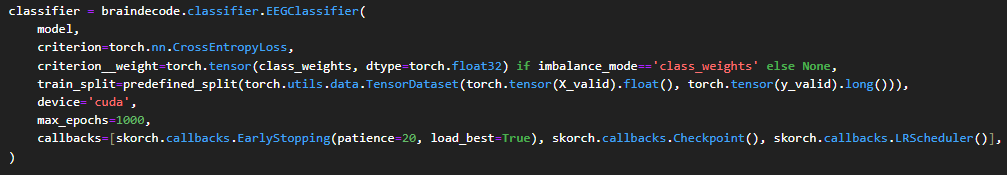
\includegraphics[width=1\linewidth]{wrapper_clasificator_braindecode.png}
    \caption{Apelarea wrapper-ului din braindecode}
    \label{fig:enter-label}
\end{figure}

La nivelul acestuia am setat loss-ul ca fiind CrossEntropyLoss din librăria pytorch \cite{pytorch}, precum și EarlyStopping și LRScheduler drept callback-uri din librăria skorch \cite{skorch}. Astfel, modelul evită overfitting-ul prin oprirea antrenării în momentul în care nu a mai progresat din punctul de vedere al loss-ului pe setul devalidare timp de 20 de epoci. De asemenea, acesta dispune și de un learning rate variabil ce îl ajută sa converarga rapid la o soluție. 

\begin{equation}
    \text{loss}(x, y) = -\frac{1}{N} \sum_{n=1}^{N} w_{y_n} \cdot \log\left(\frac{\exp(x_{n,y_n})}{\sum_{c=1}^{C} \exp(x_{n,c})}\right) \times \mathbb{1}\{y_n \neq \text{ignore\_index}\}
\end{equation}

Putem observa că formula pentru CrossEntropyLoss conține un \(w_{y_n}\). Acesta reprezintă un parametru legat de imbalansul claselor. Astfel, modelul îmi permite să abordez ambele modalități de rezolvare a problemei de balansare a claselor. Evaluarea modelelor am făcut-o asemănător cu cea a modelelor clasice, în funcție de f1-score și accuracy.

------------DE ADAUGAT GRAFIC AICI CU SCORURILE------------


\subsection{Modele personale}
Pentru a creea modele personale am utilizat keras, deoarece aduce conceptele din domeniul de Machine Learning la un nivel înalt și ușor de utilizat. Modelele mele au abordat atât paradigma învățării feature-urilor statistice și spectrale extrase din semnal, cât și a semnalului ca feature în sine.
%\chapter{Rezultate}

\section{Evaluarea performantei}
\subsection{Metrici utilizate: acuratetea, precizie, f1-score}

\section{Analiza detaliata a rezultatelor}
\subsection{Compararea performantelor intre diferite modele(graficele mele)}

\section{Grafice si interpretarea acestora}
\subsection{Curbe ROC, matricea de confuzie, etc.}

\def\timpInainteDeRay{0}
\def\timpDupaRay{0}

\chapter{Arhitectura aplicației}
\section{Împărțirea codului}
Codul este împărțit în 4 clase diferite. Ele au rolul de a forma un pipeline ce primește ca input fișiere în format csv, împreună cu montura electrozilor și ca rezultat oferă obiecte în formatul librăriei MNE.
În total, pipeline-ul meu este format din 5 clase: EEGPipelineOptions, EEGSubjectPipeline, EEGDataLoader, EEGPreprocessor și EEGEpochedData. 

Prima dată, opțiunile de preprocesare și de formatare în epoci sunt setate utilizând EEGPipelineOptions. Acest obiect este trimis mai departe către EEGSubjectPipeline. Aici, este orchestrat restul pipeline-ului în felul următor: datele din format .csv sunt transformate în format .fif(compatibil cu MNE) utilizând EEGDataLoader. Datele în format .fif sunt transformate în date de forma mne.Raw(semnalul întreg, nesegmentat). Aici sunt totodată și preprocesate utilizând filtrul bandpass, ICA, interpolarea, și/sau, opțional, normalizare și scalare în intervalul [0, 1].  Ultimul pas îl reprezintă EEGEpochedData, unde semnalul Raw este segmentat în epoci. În funcție de opțiunile alese, aici poate fi aplciat și algoritmul de AutoReject pentru a scăpa de epocile corupte. Totodată, în această clasă este situată și funcția de extragere a setului de date, împreună cu labelul acestuia.


\section{Optimizarea încărcării datelor folosind Ray}
Pentru a încărca eficient cei 26 de participanți am utilizat librăria Ray\cite{Ray}. Ray este o librărie specializată în paralelizarea programelor Python, având ca scop principal programele din domeniul de Machine Learning. Modul de paralelizare a constat prin decorarea functiilor de încarcare a datelor cu @ray.remote și așteptarea rezultatului cu ray.get. Am folosit astfel toate cele 8 core-uri de care dispune calculatorul meu. De asemenea, timpul a fost redus de la $\timpInainteDeRay$ secunde la $\timpDupaRay$ secunde.

\setlength{\abovecaptionskip}{0pt}
\setlength{\belowcaptionskip}{0pt}
\clearpage
\begin{figure}[!h]
    \centering
    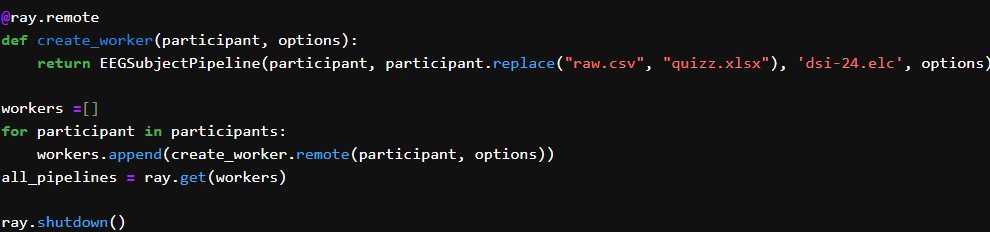
\includegraphics[width=1\linewidth]{images/ray.png}
    \caption{Paralelizare utilizând Ray}
    \label{fig:enter-label}
\end{figure}

\begin{figure}[h]
    \centering
    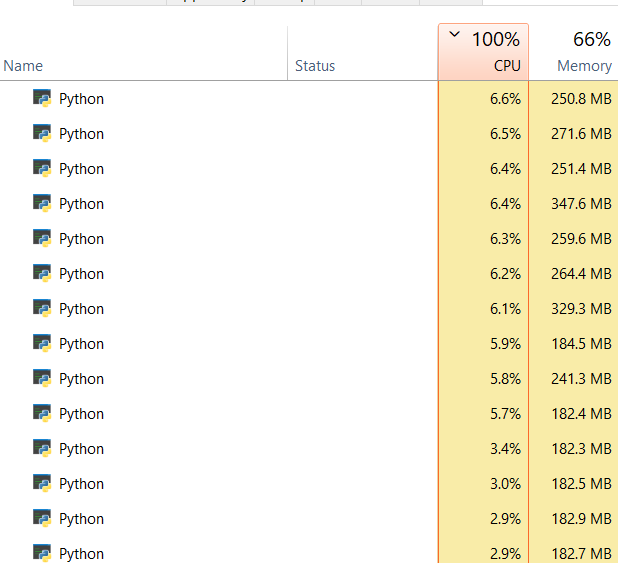
\includegraphics[width=0.7\linewidth]{task_manager.png}
    \caption{Load-ul pe calculator}
    \label{fig:enter-label}
\end{figure}
\chapter{Concluzii}

\section{Interpretarea rezultatelor}
\subsection{Ce indica performanta obtinuta}

\section{Limitarile studiului}
\subsection{Probleme intampinate: o gramada(dimensiunea setului de date, calitatea EEG-urilor}

\section{Propuneri pentru imbunatatiri viitoare}
\subsection{Colectarea unor seturi de date mai bune/mari. Reluarea experimentului}

\section{Concluzii}
\subsection{Contributii si realizari principale}

\printbibliography[heading=bibintoc]

\end{document}